\chapter{Sandpile dynamics on complex networks}


\section{Introduction and methods}
 
The aim of this task is to study the behaviour of the Bak-Tang-Wiesenfeld sandpile model (BTW) \cite{bak1987self} on complex networks, and to reproduce the main findings presented by Bonabeau \cite{bonabeau1995sandpile}, Goh et al. \cite{goh2003sandpile} and Brummitt et al. \cite{brummitt2012suppressing}. The BTW can be used to model the phenomenon of failure cascades observed in many real--world networks, and can thus aid in understanding the relationship between the architecture of a network and its robustness in the face of node failures. The first part of the task focuses on scale--free networks, where the power--law behaviour of failure cascades depends on the degree distribution. The second part focuses on interdependent networks, where the interconnection between systems can either mitigate or exacerbate failure cascades. 

The BTW is simulated here as follows: at each time step, a grain is added to a random node $i$ of the system. If the grains at any node $i$ exceed its degree $k_i$, then it becomes unstable and topples one grain to each neighbour, and an avalanche is considered to begin. For each toppled grain, there is a probability $f$ that the grain is lost, which helps avoid the overloading of the system. Then, each node is checked again for instability and the toppling is repeated in parallel until there are no more unstable nodes, and the avalanche is considered as finished. This process is repeated until a certain amount of avalanches are registered, or until a fixed amount of grains have been added to the system. Avalanches with no lost grains are termed \textit{bulk} avalanches.

Simulations are first performed on scale--free networks with degree exponents $\gamma\in(2,\infty)$ and $f=10^{-3}$. The simulations are finished after $10^6$ avalanches have been observed, and only bulk avalanches are considered for analysis. Additionally, simulations are performed on interdependent networks linked with uncorrelated Bernoulli couplings of probability $p\in[0.001, 0.5]$, with $f=10^{-2}$. These simulations are finished after $2\times10^5$ grains are added to the system. Additional details on the methodology can be found in section \ref{sec:SOC_SM} of the Supplementary Material.


\section{Results and discussion}

In general, the area of a bulk avalanche, $A$, is expected to be distributed as $p_a(A)\sim A^{-\tau}\exp(-A/s_c)$, where $s_c\sim (\langle k\rangle f)^{-1}$ is the avalanche characteristic size. Additionally, the dynamic exponent $z$ characterises the relationship between the avalanche size, $S$, and its duration, $T$, as $S\sim T^z$. From a branching process approach, these exponents are expected to depend on the degree distribution exponent $\gamma$ as $\tau=\gamma/(\gamma-1)$ and $z=(\gamma-1)/(\gamma-2)$ for $\gamma\in(2,3)$, and to have values $\tau=3/2$ and $z=2$ for $\gamma>3$. Fig. \ref{fig:tau_and_z_vs_gamma} presents the exponents $\tau$ and $z$ with respect to $\gamma$, obtained from the simulations on scale--free networks. The observed behaviour qualitatively agrees with the theoretical prediction, and the quantitative disagreement may be due to the finite size effect. 

For interdependent networks, increasing the Bernoulli link probability $p$ between subsystems can help mitigate large avalanches up to a point, $p^*$. Fig. \ref{fig:large_S_vs_p_joint_AB} presents the probability of a large avalanche $P(S_{large})$ with respect to $p$, considering both the local and inflicted avalanche size, as well as the global average. From the simulation results, the optimal link probability is $p^*\approx 0.075$, in agreement with the source material \cite{brummitt2012suppressing}.

\begin{figure}[!h]
	\begin{center}
	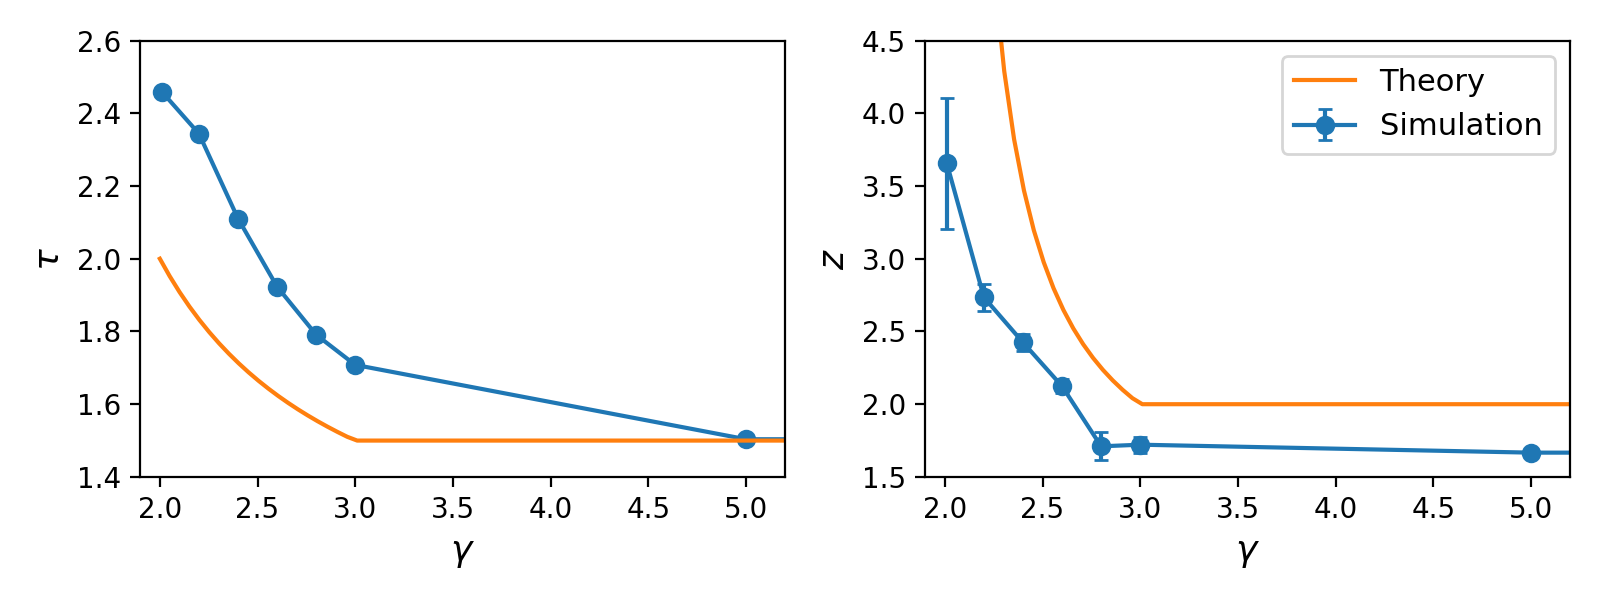
\includegraphics[scale=0.75]{./images/task_15/tau_and_z_vs_gamma.png} 
	\end{center}
	\caption{Avalanche area distribution exponent, $\tau$, (left) and dynamic exponent, $z$, (right) with respect to the degree distribution exponent, $\gamma$, of scale--free networks. The best fit from simulations is presented, alongside the theoretical prediction. \\} 
	\label{fig:tau_and_z_vs_gamma} 
\end{figure}

\begin{figure}[!h]
	\begin{center}
	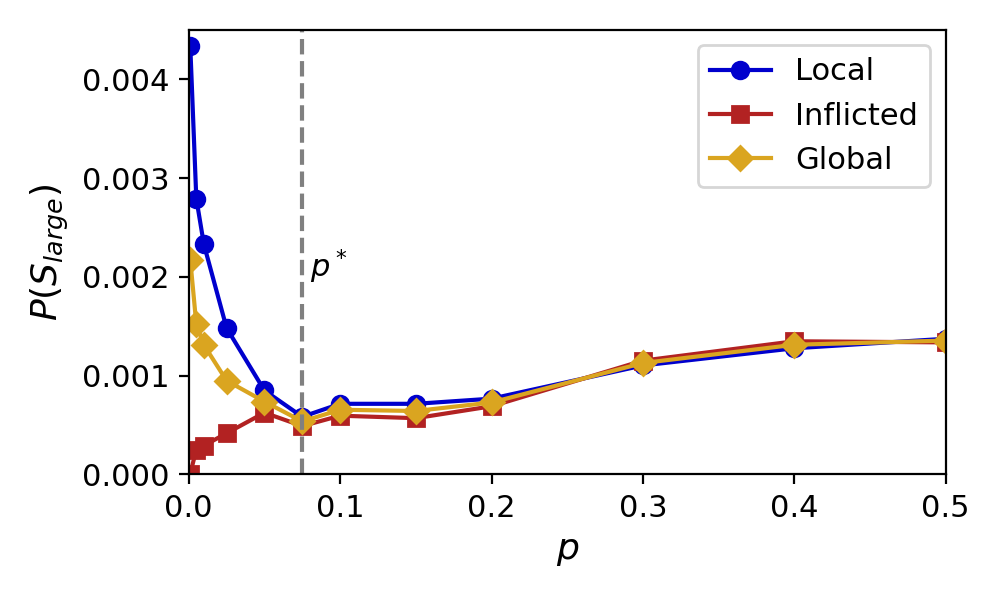
\includegraphics[scale=0.75]{./images/task_15/large_S_vs_p_joint_AB.png} 
	\end{center}
	\caption{Probability of a large avalanche, $P(S_{large})$, with respect to the link probability, $p$, for interdependent networks connected through uncorrelated Bernoulli coupling. The results for local, inflicted and global avalanches are shown, as well as the critical point $p^*$. \\} 
	\label{fig:large_S_vs_p_joint_AB} 
\end{figure}



\newpage